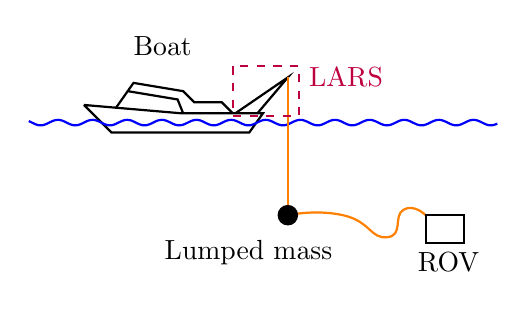
\begin{tikzpicture}[scale=0.7]
    % \draw[thick, smooth] (-.5, .5) rectangle (0, 0) node[above right] {\tiny ROV};
    % \draw[thick, smooth] (2, -1) node[above left] {\tiny ROV} rectangle (2.5, -.5);
    % \filldraw (.9, -2) rectangle (1.1, -2.2) node[below] {\tiny masse};
    % \draw[thick, blue] (0, 0) -- (1, -2) -- (2, -1);

    % Boat
    \draw[thick, black] (0,0) -- (.5,-.5) -- (3.,-.5) -- (3.25,-0.15) -- (1.75,-0.15) -- (0,0);
    \draw[thick, black] (0.583,-0.05) -- (0.9,0.4) -- (1.8,0.25) -- (2.,0.05) -- (2.5,0.05) -- (2.7,-0.15);
    \draw[thick, black] (0.8,0.25) -- (1.7,0.1) -- (1.8,-0.15) ;
    \draw[thick, black] (2.75,-0.15) -- (3.7,0.5) -- (3.15,-0.15) ;
    \node[above, xshift=1.cm, yshift=0.5cm] {Boat};
    % Surface
    \draw[thick, blue] plot[domain=-1:7.5, samples=300]  (\x,{0.05*sin(\x*10 r)-0.32}); 
    % Cable
    \coordinate (U1) at (3.7,0.5);
    \coordinate (U2) at (3.7,-2.);
    \coordinate (Ti) at (5.8, -1.9);
    \draw[thick, orange] (U1) -- (U2);
    \draw[thick, orange] plot[smooth, tension=1] coordinates{(U2) (4.7, -2.) (5.5, -2.4) (Ti) (6.2, -2)};
    \filldraw (U2) circle (5pt) node[below, xshift=-0.5cm, yshift=-0.2cm, align=left] {Lumped mass};
    \draw[thick, black] (6.2, -2) rectangle (6.9, -2.5) node[below, xshift=-0.2cm] {ROV};
    % LARS
    \draw[thick, purple, dashed] (2.7, 0.7) rectangle (3.9, -0.2) node[right, yshift=0.5cm] {LARS};

    % % Umbilical/tether
    % \draw[-latex, thick] ($(U1)!.75!(U2) + (-1,0)$) node[left, align=left] {Umbilical} -- ($(U1)!.75!(U2)$);
    % \draw[-latex, thick] ($(Ti) + (0,0.5)$) node[above, align=center] {Tether} -- (Ti);

\end{tikzpicture}